\documentclass{beamer}

\usepackage[utf8]{inputenc}
\usepackage[french]{babel}
\usepackage[T1]{fontenc}
\usepackage{graphicx}
\usepackage{geometry}
\usepackage{amssymb}
\usepackage{amsmath}
\usepackage{amsfonts}

\title{Indexer la complexité linguistique en lien avec la dynamique cérébrale à partir de signaux MEG}
\subtitle{Soutenance de stage de fin d'étude d'ingénieur}
\author{Lucas Becquet}
\institute{Ecole Centrale de Marseille}
\date{2023}

\begin{document}

\frame{\titlepage}
\setbeamertemplate{footline}[frame number]
\begin{frame}
\frametitle{Contexte}
Laboratoire de Neuroscience Cognitive de Marseille (LNC)
\center
\includegraphics[width=0.9\textwidth]{logos.png}
\end{frame}

\begin{frame}
\frametitle{Contexte}
L'équipe Développement Informatique et Infrastructure Système pour les Sciences du Cerveau (DI²S²C)
\begin{figure}[!ht]
    \centering
    \includegraphics[width=10cm]{OrganigrameDISC.png}
    \caption{Organigramme de l'équipe DISC}
    \label{fig1}
\end{figure}
\end{frame}

\begin{frame}
Peut-on discriminer des conditions expérimentales et rendre compte d'une compréhension linguistique sur la base de la quantification précise de la dynamique cérébrale ?
\end{frame}

\begin{frame}
\frametitle{Sommaire}
\tableofcontents
\end{frame}

\AtBeginSection{
  \begin{frame}
    \tableofcontents[currentsection]
  \end{frame}
}

\AtBeginSubsection{
  \begin{frame}
    \tableofcontents[currentsubsection]
  \end{frame}
}

\section{Notions de neurophysiologie}
\subsection{De l'activité neuronale aux signaux neurophysiologiques}

\begin{frame}
\frametitle{De l'activité neuronale aux signaux neurophysiologiques}
\begin{figure}[!ht]
    \centering
    \includegraphics[width=11cm]{activation_neurones.png}
    \caption{Activation neuronale. (a) Neurone seul avec représentation de sont potentiel électrique (ligne pointillée) et du champ magnétique induit (flèche bleue). (b) Groupe de neurones orientés dans le même sens, leur activation synchrone crée un champ magnétique résultant. (c) Neurones orientés de manière aléatoire, les champs magnétiques s'annulent. Adapté de Jasanof, 2007}
    \label{fig1.1}
\end{figure}
\end{frame}

\subsection{La technique d’enregistrement MEG}

\begin{frame}
\frametitle{La technique d'enregistrement MEG}
David Cohen et James Zimmerman, 1960 

Champs magnétiques de $10^{-15}$ Tesla

\begin{figure}[!ht]
    \centering
    \includegraphics[width=6cm]{fonctionnement_meg.png}
    \caption{Illustration de la MEG. Schéma d'un système MEG complet et de ses composants (issu de Dubarry, 2016)}
    \label{fig1.3}
\end{figure}
\end{frame}

\begin{frame}
\frametitle{La technique d'enregistrement MEG}
\begin{figure}[!ht]
    \centering
    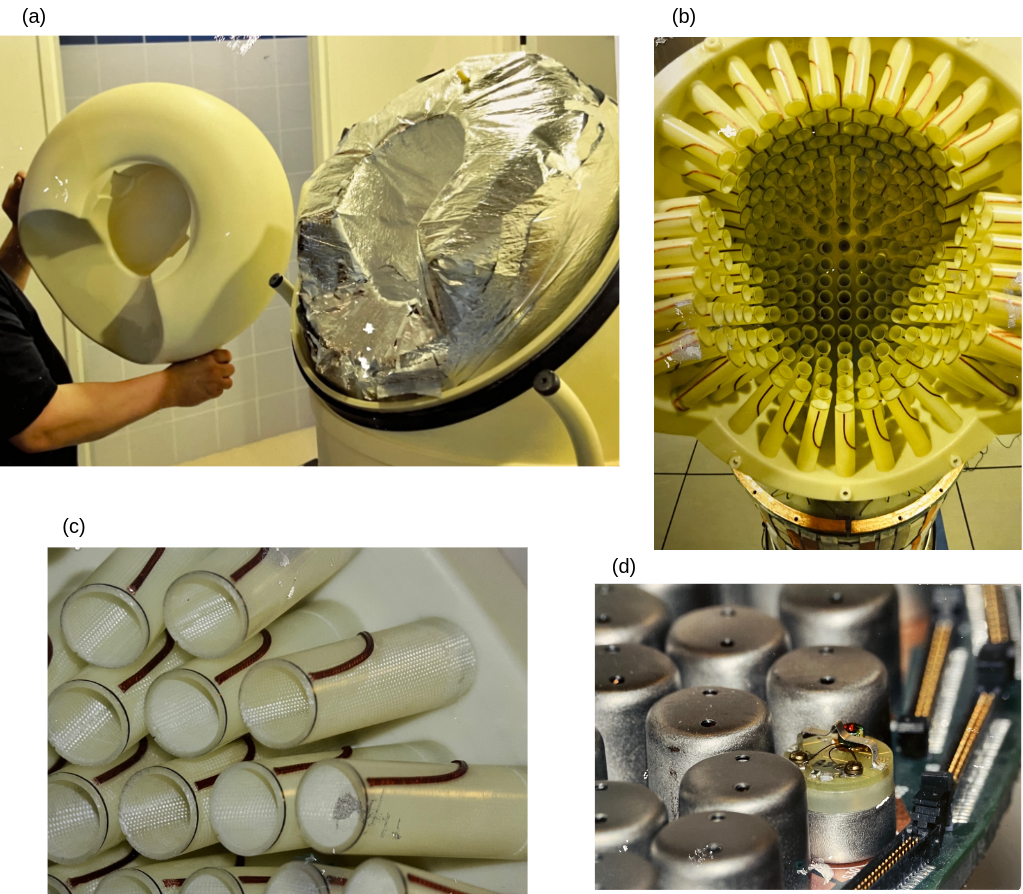
\includegraphics[width=6cm]{illustration_meg.png}
    \caption{Photographies des différents composants du système d'acquisition MEG, prises à différentes profondeurs. Centre MEG de la Timone, Marseille}
    \label{fig1.3}
\end{figure}
\end{frame}

\section{Description du dataset}
\begin{frame}
\frametitle{Description du dataset}
A 204-subject multimodal neuroimaging dataset to study language processing, Jan-Mathijs Schoffelen and Robert Oostenveld and Nietzsche H.L.Lam and Julia Uddén and Annika Hultén and Peter Hagoort, 2019.
\begin{figure}[!ht]
    \centering
    \includegraphics[width=10cm]{orga_dataset.png}
    \caption{Organisation du dataset}
    \label{fig2.1}
\end{figure}
\end{frame}

\begin{frame}
\frametitle{Description du dataset}
\begin{enumerate}
    \item 180 phrases simples appelées simple relative clause sentence (RC-)
    \item 180 phrases complexes appelées relative clause sentence (RC+)
\end{enumerate}
\begin{figure}[!ht]
    \centering
    \includegraphics[width=11cm]{stimuli.png}
    \caption{Exemple des différents stimuli : Phrase simple (RC- sentence), phrase complexe (RC+ sentence) et listes aléatoires de mots associées}
    \label{fig2.2}
\end{figure}
\end{frame}

\begin{frame}
\frametitle{Description du dataset}
\begin{figure}[!ht]
    \centering
    \includegraphics[width=11cm]{events_id.png}
    \caption{Identification des différents évènements et stimuli lors de l'enregistrement de la tâche de compréhension}
    \label{fig2.3}
\end{figure}
\end{frame}

\begin{frame}
\frametitle{Description du dataset}
\begin{figure}[!ht]
    \centering
    \includegraphics[width=11cm]{events_vis.png}
    \caption{Visualisation des différents événements au cours du temps d'un sujet de la tache visuelle}
    \label{fig3.5}
\end{figure}
\end{frame}

\section{Pré-traitement des signaux MEG}

\begin{frame}
\frametitle{Pré-traitement des signaux MEG}
MNE-Python 
\begin{figure}[!ht]
    \centering
    \includegraphics[width=11cm]{raw_info.png}
    \caption{Meta-données d'un enregistrement de la tâche de compréhension visuelle. On peut observer les différents canaux, y accéder aussi plus en détails, on voit aussi que la fréquence d'échantillonnage est de $1200 Hz$}
    \label{fig3.1}
\end{figure}
\end{frame}

\begin{frame}
\begin{figure}[!ht]
    \centering
    \includegraphics[width=11cm]{schema_pre_traitement.png}
    \caption{Protocole de pré-traitement des données MEG. (a) On applique d'abord un filtre passe-haut. (b) On applique un filtre coupe-bande. (c) On effectue la segmentation temporelle et donc la création d'époques des séries temporelles du signal MEG}
    \label{fig3.2}
\end{figure}
\end{frame}

\subsection{Séries temporelles et filtre passe-haut}

\begin{frame}
\frametitle{Séries temporelles et filtre passe-haut}
\begin{figure}[!ht]
    \centering
    \includegraphics[width=11cm]{series_temporelles_effet_hp.png}
    \caption{A gauche, séries temporelles des différents canaux du signal MEG brut. A droite, séries temporelles après application du filtre passe-haut}
    \label{fig3.3}
\end{figure} 
\end{frame}

\subsection{Spectre et filtre coupe-bande}
\begin{frame}
\frametitle{Spectre et filtre coupe-bande}
\begin{figure}[!ht]
    \centering
    \includegraphics[width=11cm]{spectre_effet_coupe_bande.png}
    \caption{Graphe de la densité spectrale relatif à l'enregistrement d'un sujet de la tâche visuelle. En haut, le spectre du signal brut. En bas, le spectre du signal une fois le filtre coupe-bande à $50 Hz$ appliqué}
    \label{fig3.4}
\end{figure}
\end{frame}

\subsection{Segmentation temporelle du signal}

\begin{frame}
\frametitle{Segmentation temporelle du signal}
\begin{figure}[!ht]
    \centering
    \includegraphics[width=09cm]{events_temporel.png}
    \caption{Visualisation des événements directement sur les différents canaux du signal temporel}
    \label{fig3.6}
\end{figure} 
\end{frame}

\section{Analyse dans le cadre de théorie de l'information}

\begin{frame}
\frametitle{Schéma de l'algorithme mis en place durant le stage}
\begin{figure}[!ht]
    \centering
    \includegraphics[width=11cm]{schema_algorithme.png}
    \caption{Schéma de l'algorithme mis en place durant le stage}
    \label{fig0.2}
\end{figure}
\end{frame}

\subsection{Représentation symbolique d'un système dynamique}

\begin{frame}
\frametitle{Représentation symbolique d'un système dynamique - Théorie}
\begin{figure}[!ht]
    \centering
    \includegraphics[width=6cm]{representation_symbolique.png}
    \caption{Illustration de la représentation symbolique dans l'espace des phases. Ici représenté en seulement 2 dimenions avec une partition binaire, les points des trajectoires à gauche de la ligne en pointillé rouge sont associés au symbole 1 tandis que ceux à droite sont associés au symbole 0.}
    \label{fig4.1}
\end{figure}
\end{frame}

\begin{frame}
\frametitle{Représentation symbolique d'un système dynamique - Pratique}
\begin{figure}[!ht]
    \centering
    \includegraphics[width=09cm]{partition_serie_temporelle.png}
    \caption{Illustration d'une équipartition par histogramme des valeurs d'une série temporelle. Exemple d'une partition à 4 symboles d'une sinusoïde. On peut identifier les différents intervalles qui correspondent chacuns à un symbole de la partition}
    \label{fig4.2}
\end{figure}
\end{frame}

\begin{frame}
\frametitle{Représentation symbolique d'un système dynamique - Pratique}
\begin{itemize}
\item <1> Matrice des données (capteurs $\times$ temps)

\item <2-> Soit $M$ la transposée de la matrice des données $m \times n$,

\item<3-> 
\begin{equation}
	M = USV^T
\end{equation}

\item<4->
\begin{enumerate}
	\item $U \in \mathcal{R}^{m \times n}$ 
	\item $S$ est une matrice diagonale de $\mathcal{R}^{n \times n}$ qui contient les valeurs propres de $M^TM$
	\item $V^T \in \mathcal{R}^{n \times n}$ 
\end{enumerate}
\end{itemize}
\end{frame}

\begin{frame}
\frametitle{Représentation symbolique d'un système dynamique - Pratique}
Critère de sélection de Schwarz
\begin{figure}[!ht]
    \centering
    \includegraphics[width=6cm]{30vp.png}
    \caption{Graphe des 30 premières valeurs propres issues de la SVD de la matrice des données pour un sujet de la tâche visuelle}
    \label{fig4.3}
\end{figure}
\end{frame}

\begin{frame}
\frametitle{Représentation symbolique d'un système dynamique - Pratique}
On ne garde donc qu'une partie $d$ des vecteurs propres contenus dans $V$ de sorte à avoir une matrice $U' \in {R}^{n \times d}$. De la même manière, on crée $S' \in {R}^{d \times n}$ en tronquant $S$ et $V' \in {R}^{n \times d}$. On obtient alors notre matrice des données réduite par $M' = U'S'V'^T$.
\begin{figure}[!ht]
    \centering
    \includegraphics[width=6cm]{representation_espace_des_phases.png}
    \caption{Espace des phases de 3 valeurs singulières avec une partition binaire}
    \label{fig4.4}
\end{figure}
\end{frame}

\subsection{Entropie}

\begin{frame}
\frametitle{Entropie}
Soit $X$ une variable aléatoire discrète ayant $\mathcal{X}$ comme alphabet.
\begin{equation}
    H(X) = - \sum_{x \in \mathcal{X}} p(x)logp(x)
\end{equation}
\begin{figure}[!ht]
    \centering
    \includegraphics[width=6cm]{exemple_entropie.png}
    \caption{Entropie $H(p)$ en fonction de la probabilité $p$ d'un événement binaire}
    \label{fig4.5}
\end{figure}
\end{frame}

\begin{frame}
\frametitle{Entropie}
\begin{block}{Théorie de l'information}
Quantité d'information produite par la source
\end{block}

\begin{alertblock}{Théorie des systèmes dynamiques}
Complexité intrinsèque du système dynamique
\end{alertblock}

\vspace{2ex}
\textcolor{green}{Informatique théorique}

\vspace{2ex}
Longueur minimale d'un code universel pour transmettre un message
\end{frame}

\subsection{Taux d'entropie et estimation}

\begin{frame}
\frametitle{Définition de l'entropie dans notre contexte}
\begin{equation}
    H_n = - \sum_{w}p_n(w)lnp_n(w)
\end{equation}

\begin{enumerate}
	\item $w$ mot de longueur n
	\item $p_n(w)$ distribution de probabilité
\end{enumerate}
\end{frame}

\begin{frame}
\frametitle{Taux d'entropie}
\begin{equation}
    h = \lim_{n \to \infty}\frac{H_n}{n} = \lim_{n \to \infty}H_{n+1} - H_n \label{eq:convergence2}
\end{equation}
\end{frame}

\begin{frame}
\frametitle{Estimateur algorithmique de Lempel-Ziv}
\begin{itemize}
\item<1->
\begin{equation}
    1 \cdot 0 \cdot 01 \cdot 11 \cdot 100 \cdot 101 \cdot 00 \cdot 010 \cdot 11... .
\end{equation}

\item<2->
\begin{equation}
    \hat{L} = \frac{\mathcal{N}_w[1 + log_k\mathcal{N}_w]}{N}
\end{equation}

\item<3-> où

\begin{equation}
    \lim_{n \to \infty} \hat{L} = \frac{h}{lnk} \label{eq:lempelziv}
\end{equation}

\begin{enumerate}
	\item $k$ taille de l'alphabet
	\item $\mathcal{N}_w$ nombre de mots du dictionnaire
	\item $N$ taille de la séquence symbolique
\end{enumerate}
\end{itemize}
\end{frame}

\section{Développement et code Python}

\begin{frame}
\frametitle{Scikits-symbolic}
Module python : fonctions, de classes et de méthodes de la théorie de l'information permettant de manipuler les séquences symboliques

\begin{figure}[!ht]
    \centering
    \includegraphics[width=4cm]{arborescence.png}
    \caption{Arborescence (de profondeur 2) du module scikits-symbolic}
    \label{fig5.1}
\end{figure}
\end{frame}

\begin{frame}
\frametitle{Tests}
Tests réalisés avec Doctest
\begin{figure}[!ht]
    \centering
    \includegraphics[width=09cm]{exemple_doctest.png}
    \caption{Exemple d'un test réalisé avec Doctest échoué volontairement}
    \label{fig5.3}
\end{figure}
\end{frame}

\begin{frame}
\frametitle{Documentation associée}
Documentation avec Sphinx
\begin{figure}[!ht]
    \centering
    \includegraphics[width=9cm]{Alphabet.png}
    \caption{Aperçu du rendu de la documentation via Sphinx}
    \label{fig5.3}
\end{figure}
\end{frame}

\section{Résultats et tests statistiques}

\begin{frame}
\frametitle{Interprétation des résultats}
On s'intéresse à la valeur p ou "p-value" comme résultat du test-t. Celle-ci nous donne la probabilité de l'hypothèse nulle, i.e., que les deux populations sont statistiquement identiques. Lorsque l'on obtient une valeur p inférieure à $5\%$, $p\geq 0.05$, on peut considérer que la probabilité de l'hypothèse nulle correspond au hasard et donc que les deux échantillons sont statistiquement différents.
\end{frame}

\subsection{Target word vs individual word}

\begin{frame}
\frametitle{Target word vs individual word}
\begin{figure}[!ht]
    \centering
    \includegraphics[width=8cm]{Targetword_vs_Individualword.png}
    \caption{Tests t apparayés entre les vecteurs d'entropie relatifs aux target words par rapport aux individual words}
    \label{fig6.1}
\end{figure}
\end{frame}

\subsection{Phrases simples vs listes aléatoires de mots issues de phrases simples}

\begin{frame}
\frametitle{Phrases simples vs listes aléatoires de mots issues de phrases simples}
\begin{figure}[!ht]
    \centering
    \includegraphics[width=8cm]{Phrases_vs_Listes_aleatoires.png}
    \caption{Tests t apparayés entre les vecteurs d'entropie relatifs aux phrases par rapport aux listes aléatoires de mots}
    \label{fig6.2}
\end{figure}
\end{frame}

\subsection{Tâche visuelle vs tâche auditive}

\begin{frame}
\frametitle{Tâche visuelle vs tâche auditive}
\begin{figure}[!ht]
    \centering
    \includegraphics[width=8cm]{visuelle_vs_auditive.png}
    \caption{Tests t apparayés entre les vecteurs d'entropie relatifs à la tâche visuelle par rapport par rapport à la tâche auditive}
    \label{fig6.3}
\end{figure}
\end{frame}

\begin{frame}
\frametitle{Conclusion et ouverture}
\begin{figure}[!ht]
    \centering
    \includegraphics[width=11cm]{p_value_significative.png}
    \caption{Valeurs p significatives des tests t. L'axe des ordonnées est en échelle logarithmique afin de pouvoir distinguer les différentes valeurs}
    \label{fig6.4}
\end{figure}
\end{frame}

\end{document}
